\chapter{Elastic Scatter of $^8$B Solar Neutrinos in SNO+}
\label{ch:es}

\section{Introduction}
\label{sec:solar:intro}

This analysis aims to measure the flux of $^8$B solar neutrinos by identifying
elastic scatter (ES) events in the water phase of SNO+.
This is achieved with a one dimensional fit to the projection of reconstructed
event direction onto the direction of the sun at the time of each event
$\cos{\theta_{sun}}$.
As shown in Figure \ref{fig:solar:backgrounds} all backgrounds are flat in
$\cos{\theta_{sun}}$ so a flat background is included in the fit, with the ES
signal shape determined from monte-carlo.
In addition to measuring the flux, this is a cross-check of the angular
resolution of SNO+ showing that the solar monte-carlo agrees with solar data.

\begin{figure}
\centering
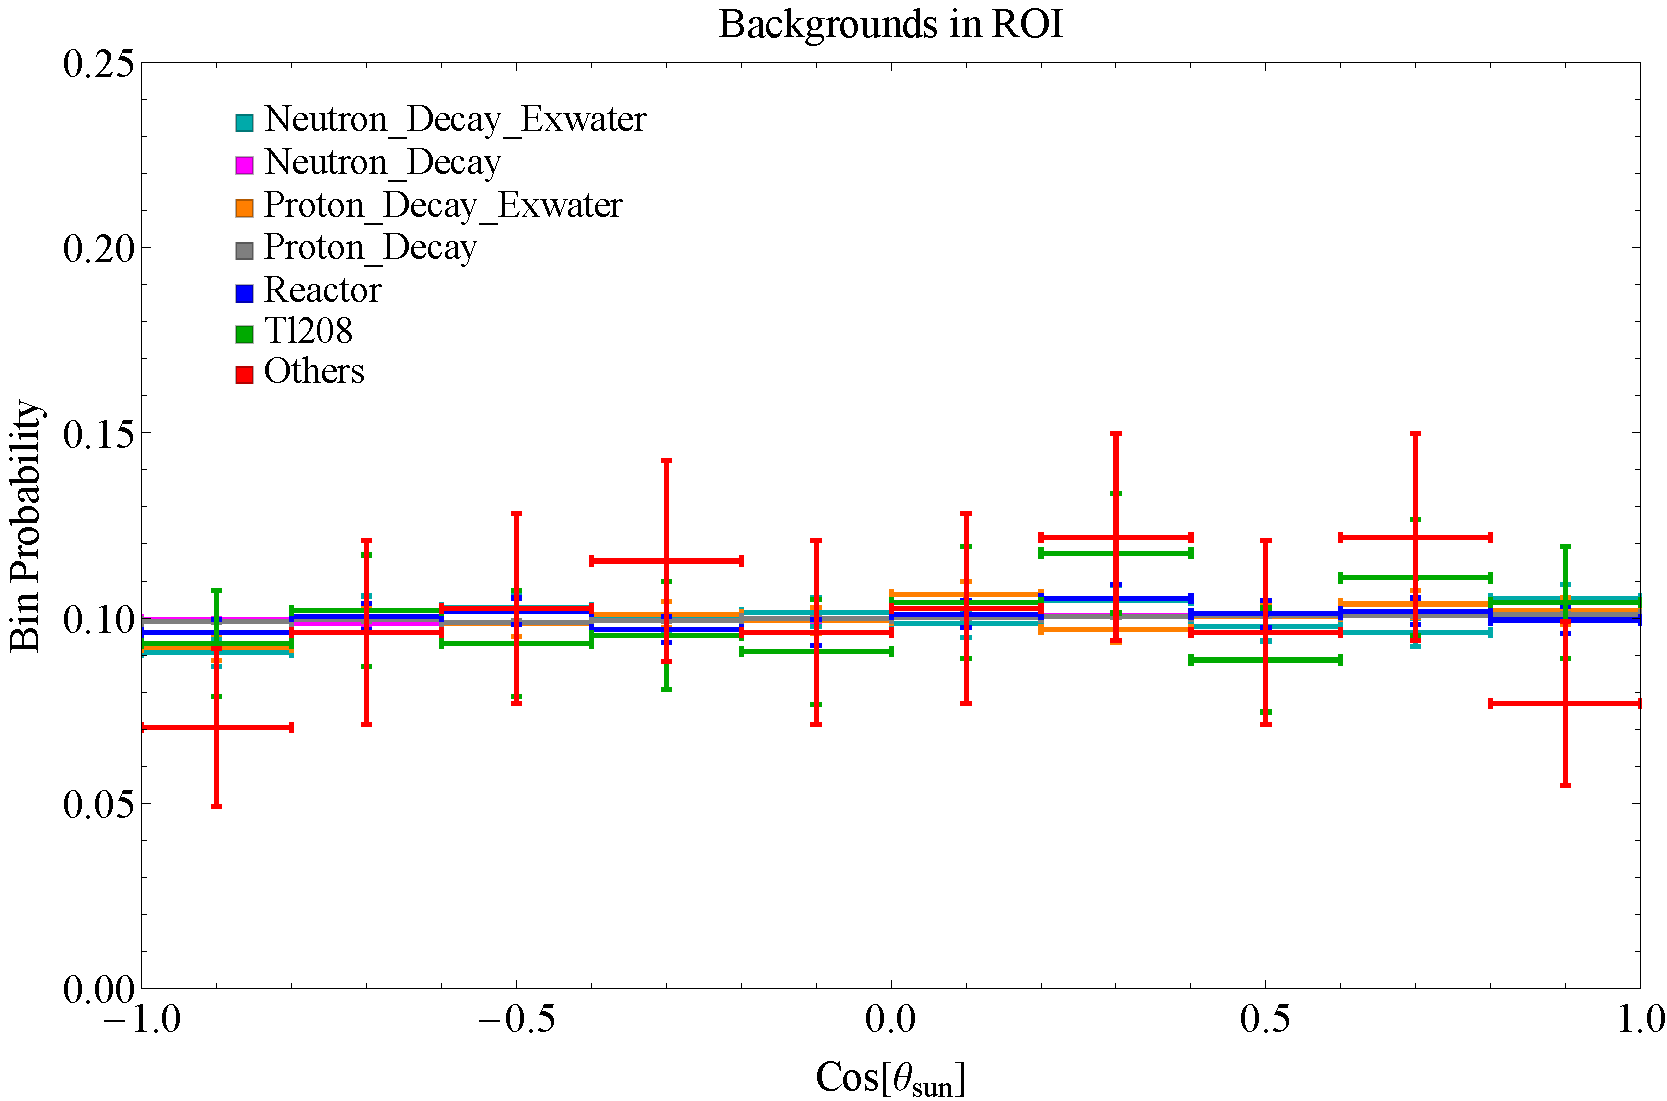
\includegraphics[width=\textwidth]{backgrounds_roi}
\caption{Backgrounds shown binned in the observable $\cos{\theta_{sun}}$ after
         solar analysis cuts are applied. Note that backgrounds with fewer than
         100 counts were combined and shown as as other.}
\label{fig:solar:backgrounds}
\end{figure}

\section{Solar Signals}
\label{sec:solar:inputs}

The SNOMAN MC from SNO is replaced by RAT MC for SNO+, however both operate very similarly.
Both $\nu_e$ and $\nu_a$ ($\nu_\mu$ and $\nu_\tau$) events generated with a known
flux and flat ($100\%$) survival/transition probability are the primary input to this
analysis.
RAT is trusted to properly simulate the $^8$B spectrum weighted by the ES cross
section and compute the total number of electrons (correct event rate) such
that the MC can be reweighted by some survival probability with
$P_{ee}+P_{ea}=1$ and, with ROI cuts applied, accurately predict the number of
expected events.
RAT MC was generated with the $^8$B flux from BS05(OP), but this was rescaled 
to a more up-to-date measured value \cite{GlobalSolarFlux}.
livetime between MC and data.
RAT is additionally trusted to correctly calculate the solar angle at any
event time.

The other main input to this analysis are MSW survival probability curves.
The code from the neutrino lifetime analysis presented earlier was levereged here to produce survival probabilities corresponding to the most up-to-date neutrino parameters available.
Physical constants and mixing parameters from PDG2016 are used in the MSW
calculation, and the $^8$B production regions and solar electron densities come
from BS05(OP).
Normal mass hierarchy is assumed.
The curves are obtained with a 3$\nu$ calculation that numerically diagonalizes
the MSW Hamiltonian at a given electron density to find the projection of
electron neutrinos onto the matter eigenstates at that density.
These matter eigenstates are then assumed to adiabatically evolve into vacuum
eigenstates as they propagate through the sun, maintaining their initial
projections.
Finally, the projections onto the vacuum eignestates are detected incoherently
at Earth (with no regeneration of coherence in the Earth) as e, $\mu$, and
$\tau$ neutrinos.
This calculation is done in 0.1 MeV intervals and is averaged over the electron
densities of the sun weighted by the $^8$B production regions.
These curves are shown in Figure \ref{fig:solar:msw}.

\begin{figure}
\centering
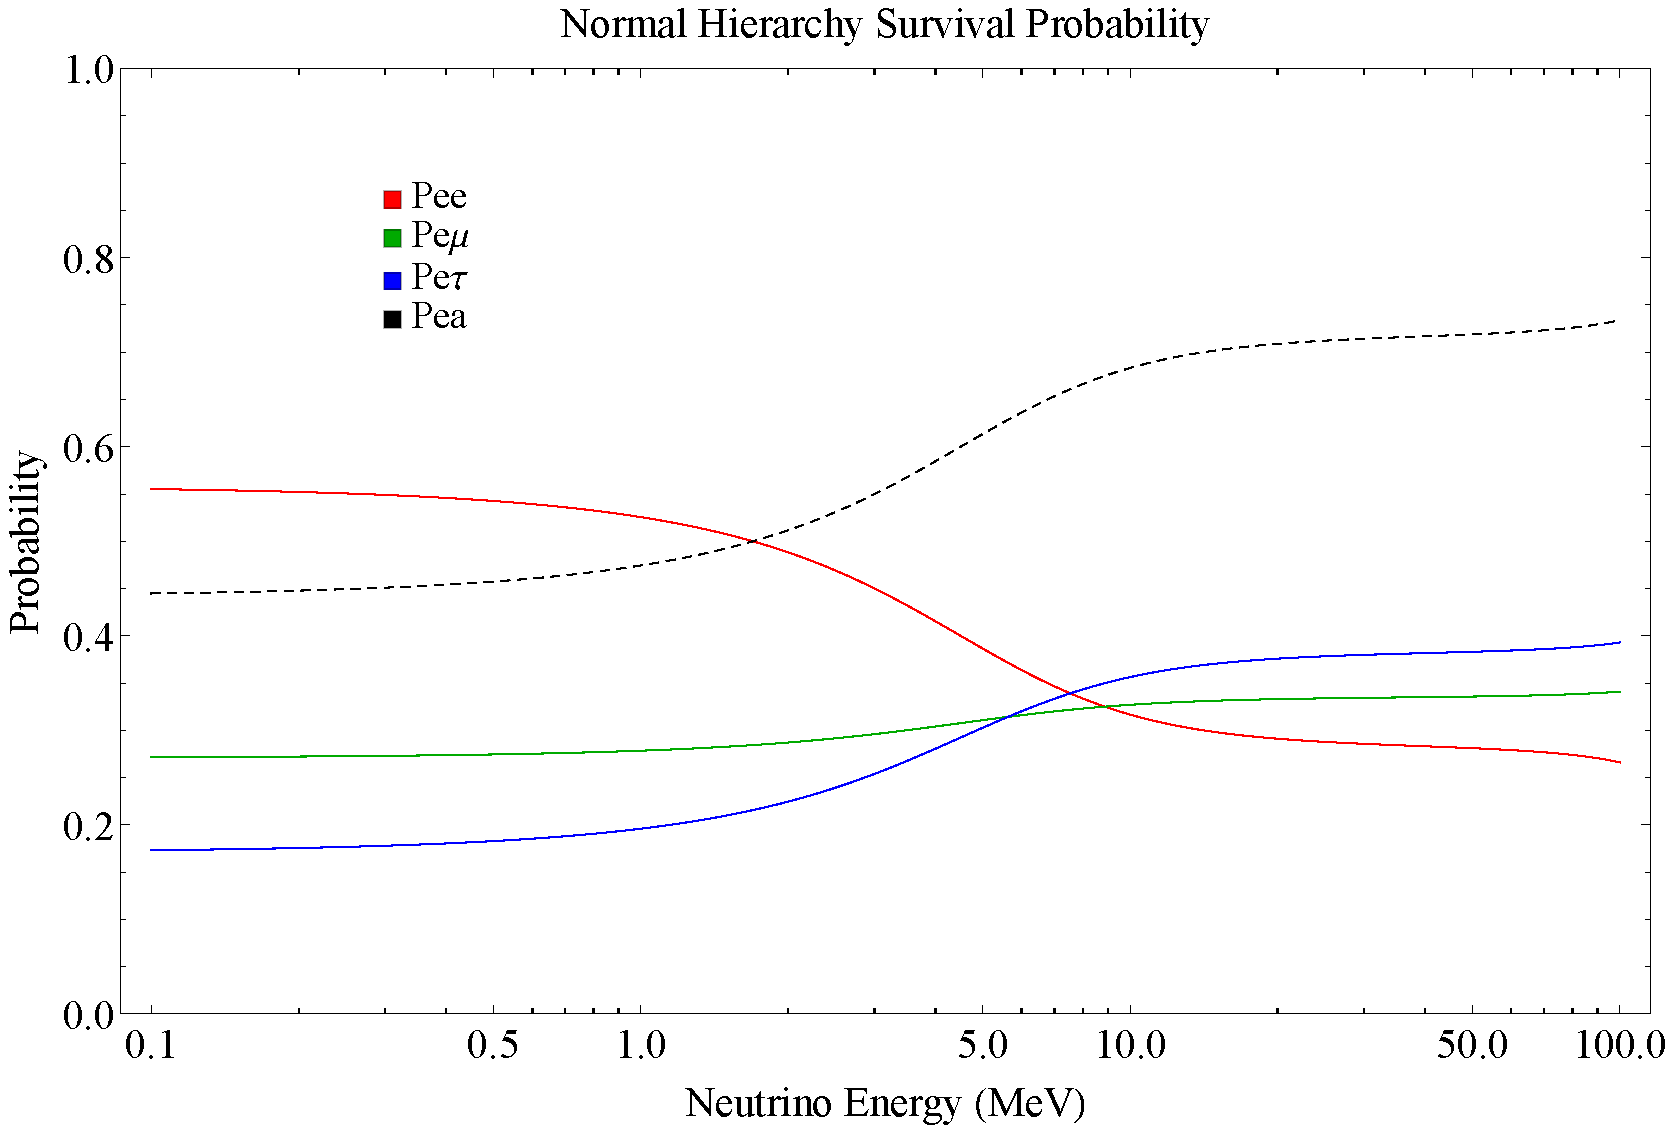
\includegraphics[width=\textwidth]{normal_survival_b8density}
\caption{The MSW survival probability curves used in the open data analysis.}
\label{fig:solar:msw}
\end{figure}

\section{Open Data Analysis}
\label{sec:solar:opendata}

To understand detector data, constrain backgrounds, and aid in the development of analyses, SNO+ provided about 16 days of detector livetime with no blinding applied.
The remaining data was withheld until analyses were developed and demonstrated to be unbiased. 
The following sections describe the development of this analysis on this open data.
Note that this was a preliminary step in the analysis, and as such not all constraints for systematic uncertanties were available.

\subsection{Analysis Cuts}
\label{sec:solar:open_cuts}

The SNO+ trigger system records a 32 bit integer where each bit is a boolean mask of the state of the trigger system for each event.
This trigger word identifies, at a very low level, what caused the detector to take data.
Low level event selection requires that the trigger word include a physics trigger based on the number of coincidentally hit PMTs, and excludes any externally forced triggers that may be in the data.
The following expression evaluates to logical false for selected events.

\begin{verbatim}
!(trig_word & 0x3F) || (trig_word & 0xBFF9400)
\end{verbatim}

Various data cleaning classifiers are run over the raw data as part of reconstruction, with the goal of identifying instrumental backgrounds or other non-physics events.
These classifiers produce another 32 bit word which can be checked for event quality.
A check of the data cleaning word requires that all standard data cleaning classifiers did not mark the event as dirty using the analysis mask 0x7FFE.
The following expression evaluates to logical false for selected events.

\begin{verbatim}
((dc_applied & ANALYSIS_MASK) & dc_flagged ) != (dc_applied & ANALYSIS_MASK)
\end{verbatim}

A valid reconstruction result is then required, meaning the reconstruction algorithms successfully converged to some value.
High level cuts are applied on the in time ratio (ITR) and isotropy ($\beta_{14}$).
The ROI is then selected with cuts on energy and radius.
Other analyses of this data identified a region of high radioactivity near the top of the detector, and for this a z dependent radial cut was adopted.
These high level cuts are summarized per time bin in Table \ref{tbl:solar:roi}.

\begin{table}[]
\begin{center}
\begin{tabular}{c|c|c}
Open & External Hotspot & Steady State  \\ \hline
100000-100399 & 100400-102048 & 102049-103402 \\ \hline
ITR $ >= 0.55$ & ITR $ >= 0.55$ & ITR $ >= 0.55$ \\
$-0.12 <= \beta_{14} <= 0.95$ & $-0.12 <= \beta_{14} <= 0.95$ & $-0.12 <= \beta_{14} <= 0.95$ \\
$5.5 <= E <= 9.0$ & $5.5 <= E <= 9.0$ & $5.5 <= E <= 9.0$ \\
$R <= 5.3$ & $R <= 5.3$ (for Z$<$0) & $R <= 5.3$ \\
 & $R <= 4.2$ (for Z$>$0) & \\
\end{tabular}
\\[2\baselineskip]
\begin{tabular}{c|c|c}
AV 1 \& 2 & AV 3 \& 4 & Post-Bubble \\ \hline
103411-105171 & 105493-105661 & 106716- \\
& 106070-106499 & \\ \hline
ITR$ >= 0.55$ & ITR$ >= 0.55$ & ITR$ >= 0.55$ \\
$-0.12 <= \beta_{14} <= 0.95$ & $-0.12 <= \beta_{14} <= 0.95$ & $-0.12 <= \beta_{14} <= 0.95$ \\
$5.5 <= E <= 9.0$ & $5.5 <= E <= 9.0$ & $5.5 <= E <= 9.0$ \\
$R <= 5.3$ & $R <= 5.3$ & $R <= 5.3$ \\
\end{tabular}
\caption{The cuts used in the open solar neutrino analysis. Selected events will pass these cuts.}
\label{tbl:solar:roi}
\end{center}
\end{table}

\begin{table}
\centering
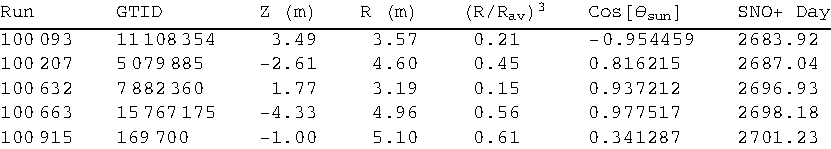
\includegraphics[width=\textwidth]{events}
\caption{The events selected by solar analysis cuts in the open dataset.}
\label{tbl:solar:openev}
\end{table}

There are 5 candidate ES events selected by the analysis cuts which are shown
with various parameters in Table \ref{tbl:solar:openev}.
The SNO+ date for the runs included along with the 5 selected events is shown
in Figure \ref{fig:solar:opendata}.
The time of day of each event along with the total number of runs at that time
is shown in Figure \ref{fig:solar:tod}.

\begin{figure}
\centering
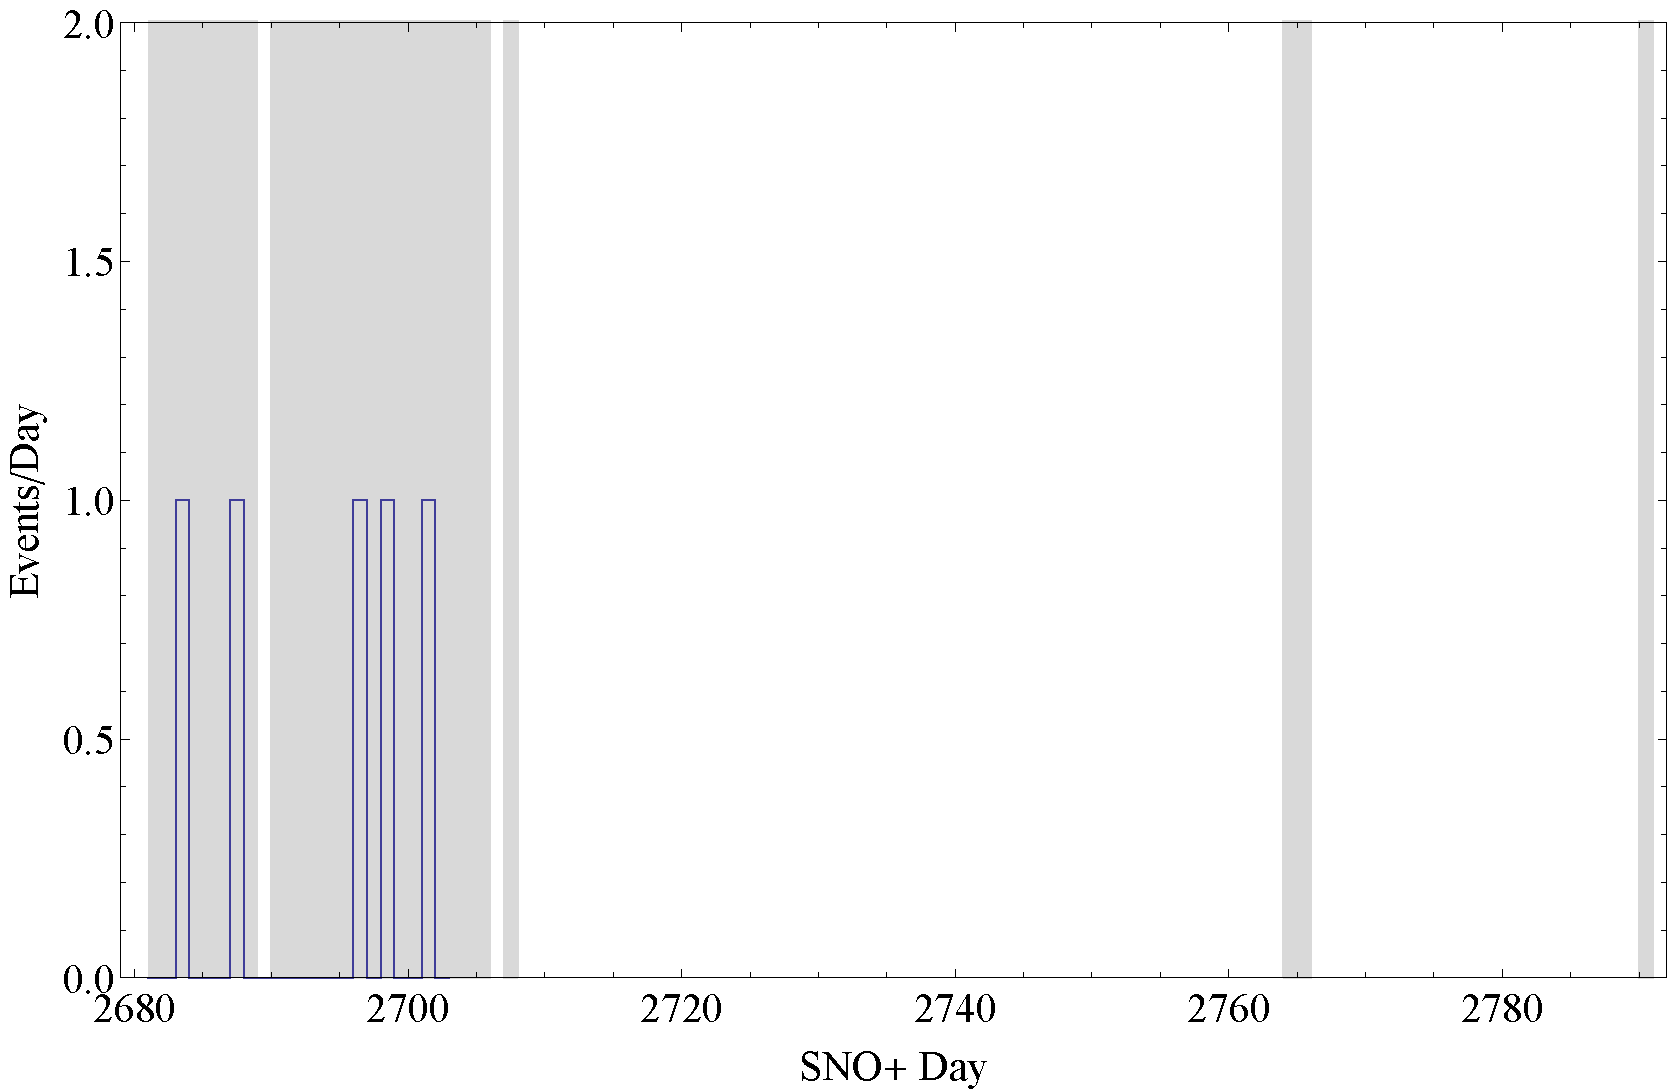
\includegraphics[width=\textwidth]{per_day}
\caption{The SNO+ days that are included in the open data analysis are shown
         shaded gray.
         The date of each selected event in the open data analysis is also shown.}
\label{fig:solar:opendata}
\end{figure}


\begin{figure}
\centering
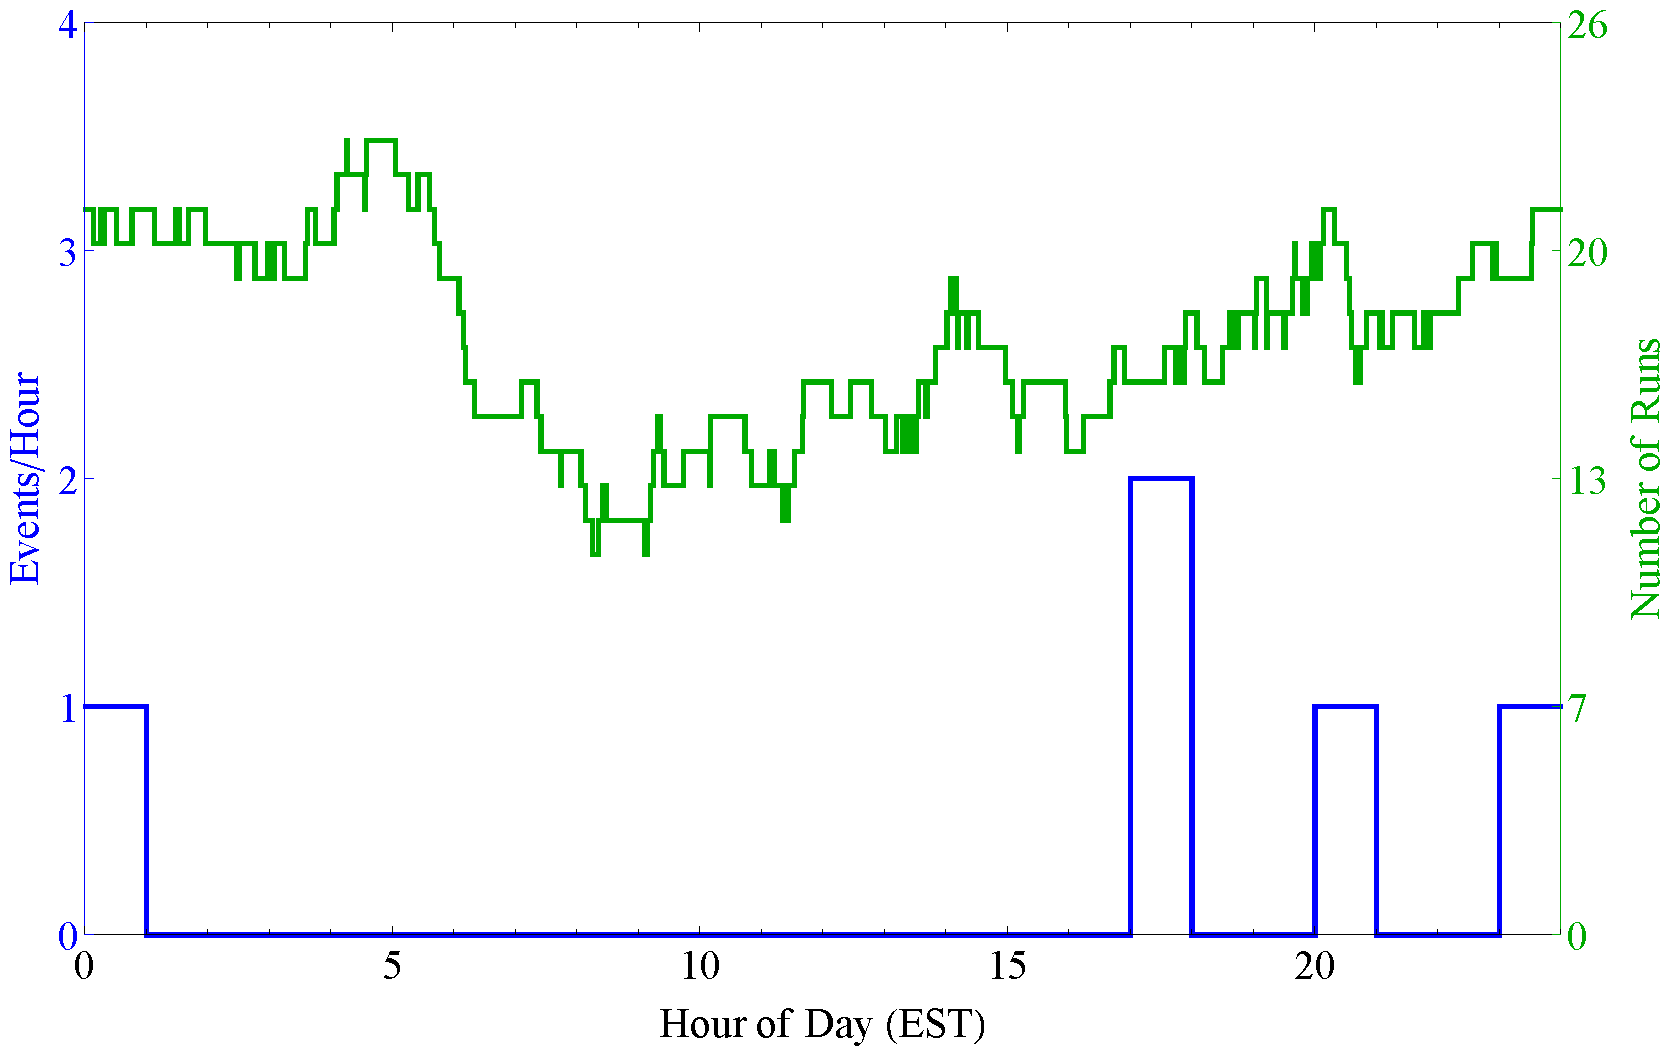
\includegraphics[width=\textwidth]{hour_of_day}
\caption{The time of day (Sudbury timezone, no DST correction) of each selected
         event in the open data analysis.
         Also shown are the number of runs at any particular time of day.}
\label{fig:solar:tod}
\end{figure}

\subsection{PDF Generation}

The MC for $\nu_e$ and $\nu_a$ events passing cuts are added to separate
$\cos{\theta_{sun}}$ histograms and weighted by the survival probability at the
true neutrino energy.
These histograms are binned at intervals of $0.2$ and normalized by MC livetime.

The MC for $\nu_e$,$\nu_a$ events are respectively generated at 1700, 9600 times
the nominal flux of $5.69\times10^{6}$ cm$^{-2}$s$^{-1}$, and each histogram is
scaled by the inverse of these flux scales.

The generated flux is the BS05(OP) prediction for $^8$B neutrinos which is a
rather old model and perhaps not the best nominal flux. 
A recent combined analysis of past solar neutrino experiments finds 
$5.16^{+0.13}{-0.09}\times10^6$ cm$^{-2}$s$^{-1}$ \cite{GlobalSolarFlux} as the 
most probable $^8$B flux.
To that end, the histogram is further scaled by the ratio of these two fluxes.
By integrating these histograms and scaling by the data livetime, the total
number of expected ES events in the ROI for the open data is calculated to be
$6.08$ events.

The $\nu_e$,$\nu_a$ histograms are added together and normalized to obtain the
total ES histogram.

\subsection{Central Fit}

With the data binned in the same way as the PDFs, $0.2$ $\cos{\theta_{sun}}$ intervals, a
$\chi^2$ fit is performed to the number of background events using a flat
histogram and the number of signal events using the normalized ES histogram.
For the open dataset, a flux scale of $0.54\pm0.37$ (stat.) $^{+0.09}_{-0.05}$ 
(syst.) is found.
Systematic uncertainties are discussed in the following section.
This fit is shown plotted with the binned data in Figure \ref{fig:solar:openfit}.

\begin{figure}
\centering
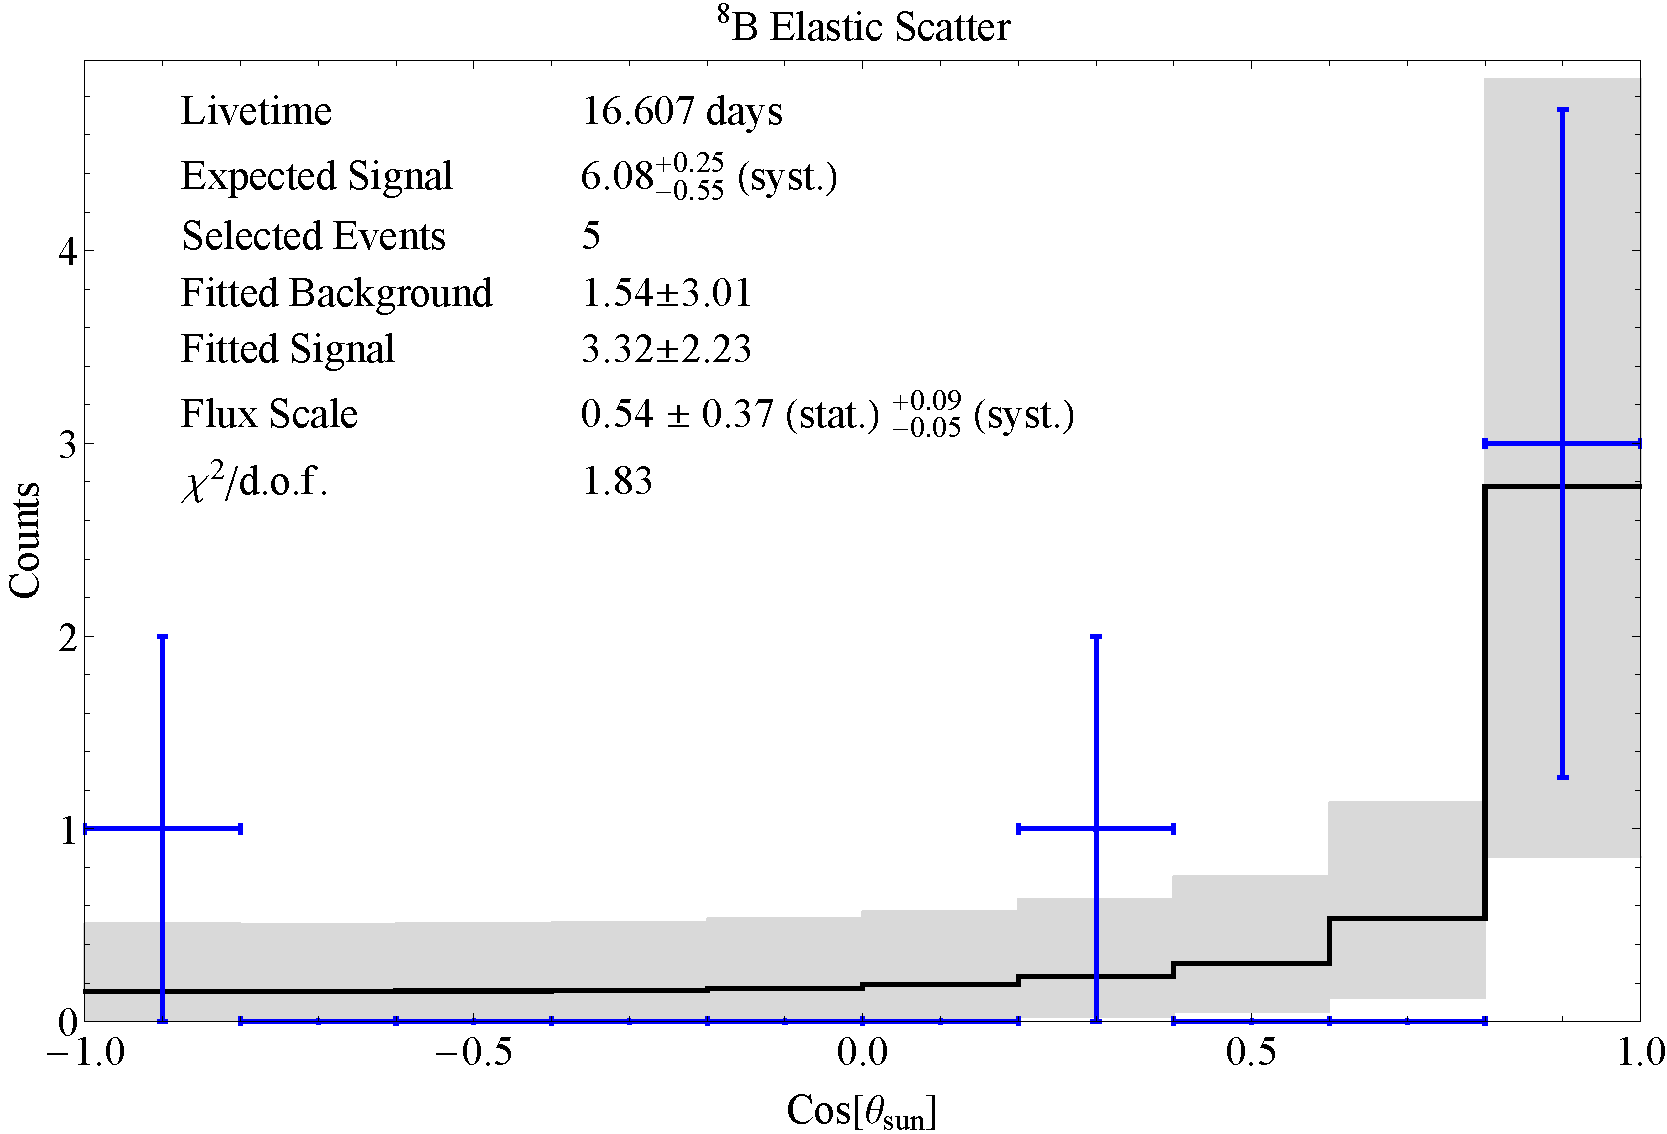
\includegraphics[width=\textwidth]{b8_es_fit}
\caption{Summary plot of the $^8B$ ES fit on the open dataset.
         The shaded regions show the fit uncertainty, with the selected events
         shown in blue.}
\label{fig:solar:openfit}
\end{figure}

\subsection{Systematic Effects}
Systematics considered here include: energy scale, energy resolution, position 
scale, position resolution, and direction resolution.
These are estimated from analyses of SNO+ calibration data, primarily from the $^{16}$N source.
As of writing, input values for position scale and direction resolution are not
available, so these uncertainties are omitted from this segment of the analysis.

Energy scale uncertainty was determined to be $0.75\%$. To evaluate the impact,
MC reconstruced energies were scaled up and down by this amount, the MC histograms 
were recreated using the nominal ROI, and the expected number of signal events 
were compared to the nominal (unscaled energy) case. The uncertainty on the 
expected number of events was determined to be $^{+0.05}_{-0.06}$.

Energy resolution was determined to be $21.0^{+5.0}_{-9.2}\%$ at 5MeV.
Following the suggested method for propagating this systematic, a gaussian smear is applied to the MC truth electron energies
and the expected number of events is compared between the nominal resolution to the worst and best case resolution. In 
only this case, the smeared MC truth energy is substituted for the MC reconstructed
energy when applying ROI cuts. The smearing applied as a function of energy is
$E_{res\,E} = E_{res\,5MeV} \sqrt{(5 MeV) \times E}$. The shift in the expected 
number of events after creating MC histograms with the nominal ROI is taken as 
the systematic effect $^{+0.25}_{-0.55}$.


Position resolution was determined to be approximately $10$cm. This analysis
is in flux as of writing, but this approximate value is expected to be near
the final number. A gaussian smear was applied to MC reconstructed positions 
and the event radius was recomputed from these smeared values. Finally the MC 
histogram was recreated to count the number of expected events. There was no 
significant effect on the expected number of events. This process was repeated
with many random seeds, and still no significant effect was seen. This is not
unexpected as this systematic moves events in and out of the ROI in a symmetric
fashion.

Direction resolution will be applied by remapping the $\cos{\theta_{sun}}$ 
observable using the Equation \ref{solar:eq:dirres}. Where $\Delta$ is either
determined from an analysis of N16 data or floated in the fit. Since this 
systematic does not affect the ROI, it will be applied directly to the MC 
histogram prior to/during the fit and will be an uncertainty on the fitted
number of events. Given the few number of events in the open data and pending
N16 analysis this has not yet been considered.

\begin{equation}
\cos{\theta'_{sun}} = 1 + \frac{\cos{\theta_{sun}}-1}{1\pm\Delta}
\label{solar:eq:dirres}
\end{equation}

The systematic effects are summarized in Table \ref{tbl:solar:systben}

\begin{table}[]
\begin{center}
\begin{tabular}{c|c|c}
Systematic & Input & Impact \\ \hline
$E_{scale}$		& $0.75\%$ & $^{+0.05}_{-0.06}$  \rule{0pt}{2.6ex}\rule[-1.2ex]{0pt}{0pt}  \\
$E_{res}$		& $21^{+5.0}_{-9.2}\%$ at 5MeV & $^{+0.25}_{-0.55}$  \rule{0pt}{2.6ex}\rule[-1.2ex]{0pt}{0pt}  \\
${XYZ}_{scale}$	& Pending &  \rule{0pt}{2.6ex}\rule[-1.2ex]{0pt}{0pt}  \\
${XYZ}_{res}$		& 10cm (approx) & $\pm0.00$  \rule{0pt}{2.6ex}\rule[-1.2ex]{0pt}{0pt}  \\
Dir$_{res}$ 	& Pending & \rule{0pt}{2.6ex}\rule[-1.2ex]{0pt}{0pt}  \\ \hline
Total			& --- &  --- \rule{0pt}{2.6ex}\rule[-1.2ex]{0pt}{0pt}  
\end{tabular}
\caption{Systematic effects considered on the open data analysis.}
\label{tbl:solar:systben}
\end{center}
\end{table}

\subsection{Alternative ROI}

There is interest in opening up the energy ROI for this analysis to include as many solar events as possible.
To that end, two alternative energy ranges are considered: 4.5 MeV to 15 MeV and 5.5 MeV to 15 MeV.
Performing an identical analysis as above but with these larger energy ROIs yields the results in Figure \ref{fig:solar:open45} and \ref{fig:solar:open55}.

\begin{figure}
\centering
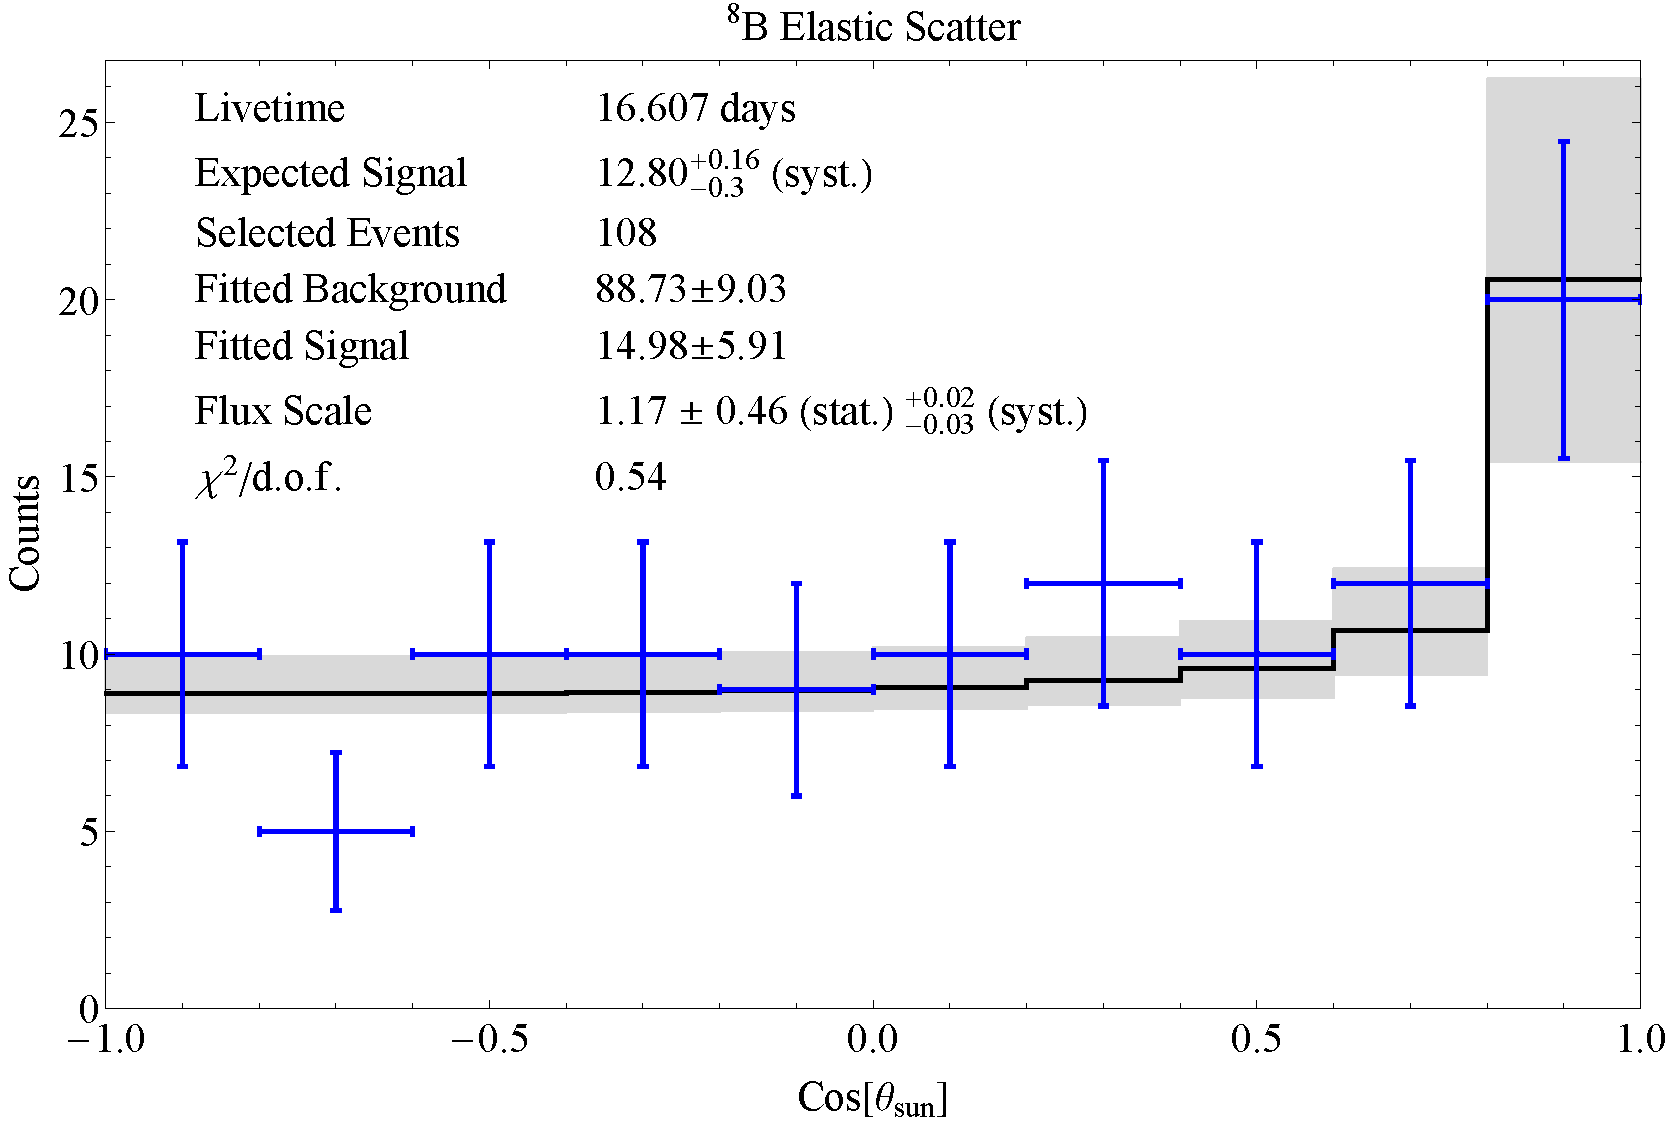
\includegraphics[width=\textwidth]{b8_es_fit_4_5}
\caption{
Summary plot of the $^8B$ ES fit on the open dataset using the alternative energy range 4.5-15.0 MeV.
The shaded regions show the fit uncertainty, with the selected events shown in blue.
}
\label{fig:solar:open45}
\end{figure}

\begin{figure}
\centering
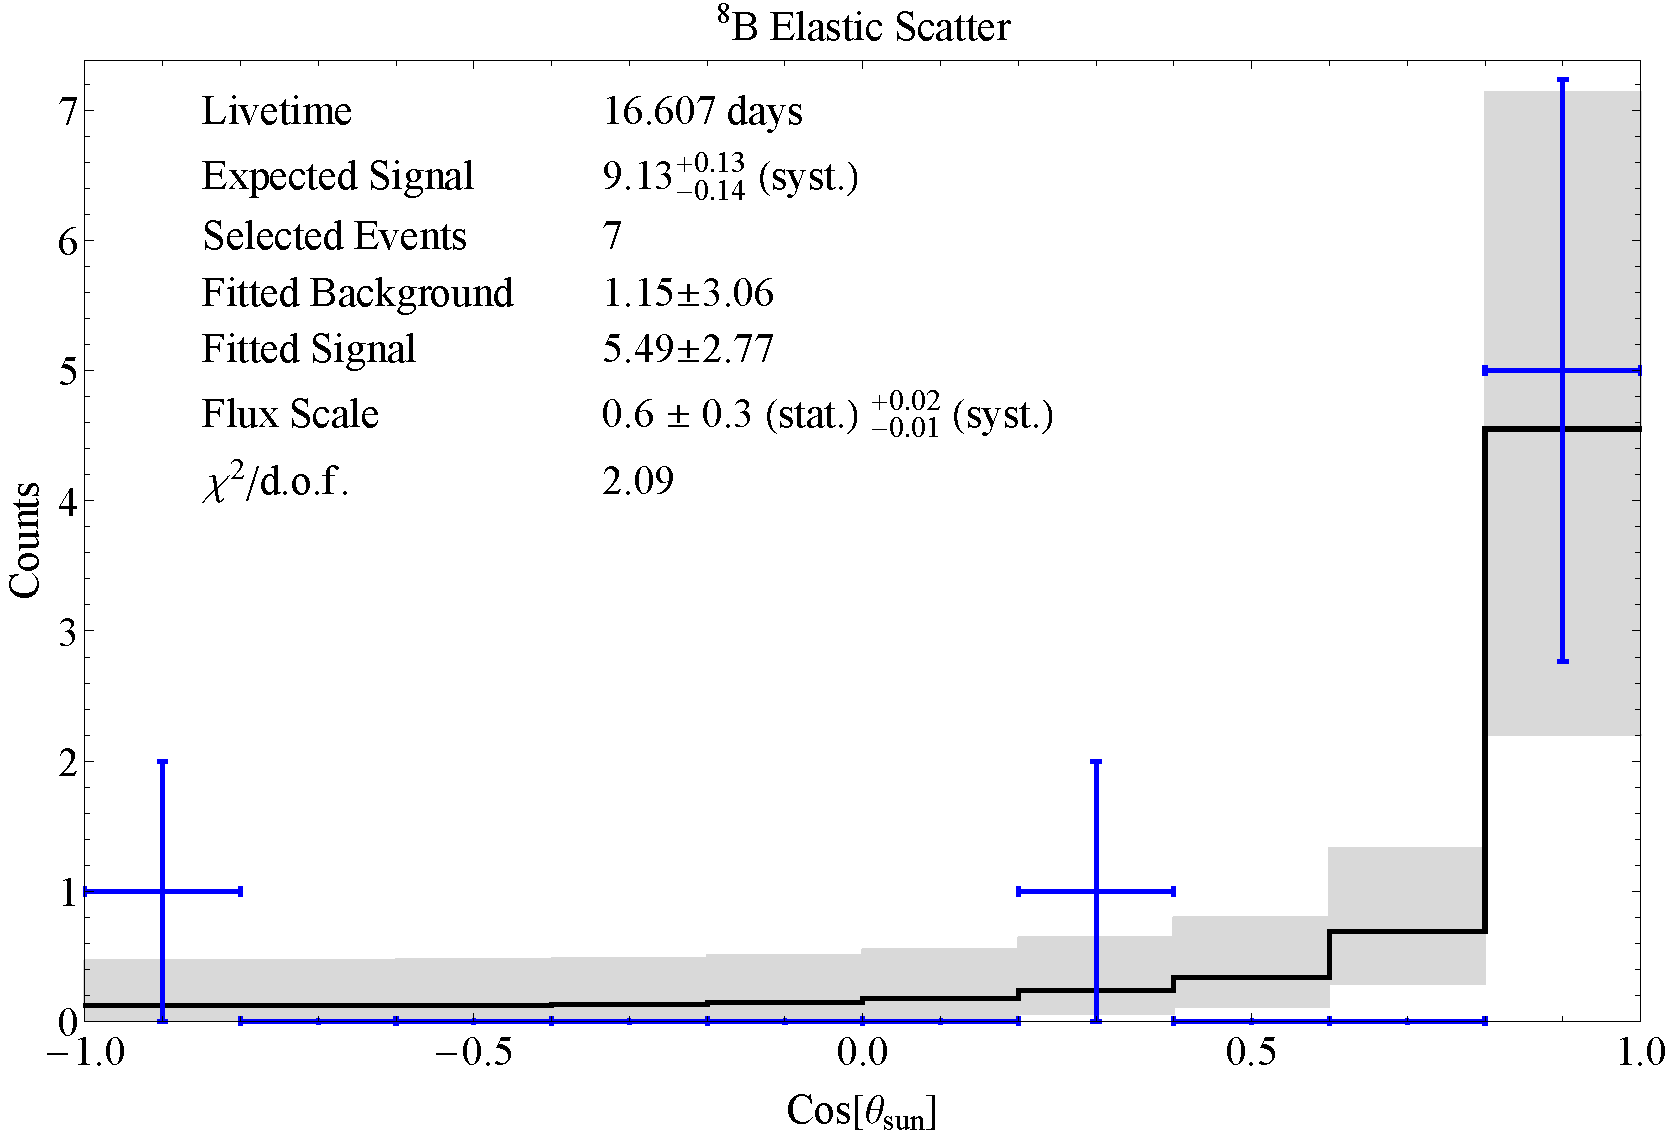
\includegraphics[width=\textwidth]{b8_es_fit_5_5}
\caption{
Summary plot of the $^8B$ ES fit on the open dataset using the alternative energy range 5.5-15.0 MeV.
The shaded regions show the fit uncertainty, with the selected events shown in blue.
}
\label{fig:solar:open55}
\end{figure}

\section{Unblinded Analysis}
\label{sec:solar:unblinded}

Following a review of the open data analysis as described in the previous section, the SNO+ Analysis Committee approved the analysis procedure to move ahead with the entire SNO+ water phase dataset.
These sections describe refinements made to the analysis and updated constraints from the systematic analyses of SNO+ water data.
Most notably, the additional livetime (approximately 114 days) and additional events this implies allows for finer data binning, and the underlying fit was changed to be a Poisson likelihood rather than a $\chi^2$ fit.

\subsection{Analysis Cuts}
\label{sec:solar:unblind_cuts}

Low level event selection requires that the trigger word include a physics
trigger and excludes any external triggers.
Compared to the open data analysis, the EXT6 trigger (bit 20) indicating 
that the 10MHz clock is not working is allowed for two reasons: there is no
livetime cut to account for this condition, and the time of the event is 
known to sufficient precision for there to be no significant effect on the 
solar direction.
The following expression evaluates to logical false for selected events.

\begin{verbatim}
!(trig_word & 0x3F) || (trig_word & 0xBEF9400)
\end{verbatim}

A check of the data cleaning word requires that all standard data cleaning
classifiers did not mark the event as dirty using the analysis mask 
0xFB0000017FFE.
The following expression evaluates to logical false for selected events.

\begin{verbatim}
((dc_applied & ANALYSIS_MASK) & dc_flagged ) != (dc_applied & ANALYSIS_MASK)
\end{verbatim}

A valid water fitter result is then required.
High level cuts are applied on the in time ratio (ITR) and isotropy ($\beta_{14}$).
The ROI is then selected cuts on energy and radius.
These high level cuts are summarized per time bin in Table \ref{tbl:solar:unblind_roi}.

\begin{table}[]
\begin{center}
\begin{tabular}{c|c|c}
Open & External Hotspot & Steady State  \\ \hline
100000-100399 & 100400-102048 & 102049-103402 \\ \hline
ITR $ >= 0.55$ & ITR $ >= 0.55$ & ITR $ >= 0.55$ \\
$-0.12 <= \beta_{14} <= 0.95$ & $-0.12 <= \beta_{14} <= 0.95$ & $-0.12 <= \beta_{14} <= 0.95$ \\
$4.5 <= E <= 15.0$ & $4.5 <= E <= 15.0$ & $4.5 <= E <= 15.0$ \\
$R <= 5.3$ & $R <= 5.3$ (for Z$<$0) & $R <= 5.3$ \\
 & $R <= 4.2$ (for Z$>$0) & \\
\end{tabular}
\\[2\baselineskip]
\begin{tabular}{c|c|c}
AV 1 \& 2 & AV 3 \& 4 & Post-Bubble \\ \hline
103411-105171 & 105493-105661 & 106716- \\
& 106070-106499 & \\ \hline
ITR$ >= 0.55$ & ITR$ >= 0.55$ & ITR$ >= 0.55$ \\
$-0.12 <= \beta_{14} <= 0.95$ & $-0.12 <= \beta_{14} <= 0.95$ & $-0.12 <= \beta_{14} <= 0.95$ \\
$4.5 <= E <= 15.0$ & $4.5 <= E <= 15.0$ & $4.5 <= E <= 15.0$ \\
$R <= 5.3$ & $R <= 5.3$ & $R <= 5.3$ \\
\end{tabular}
\caption{The cuts used in the unblinded solar neutrino analysis. Selected events will pass these cuts.}
\label{tbl:solar:unblind_roi}
\end{center}
\end{table}

\subsection{Fit Strategy}
\label{sec:solar:fit_strategy}

The MC for $\nu_e$ and $\nu_a$ events passing cuts are added to separate
$\cos{\theta_{sun}}$ histograms and weighted by the survival probability at the
true neutrino energy.
These histograms are binned at intervals of $0.05$.

The MC for $\nu_e$,$\nu_a$ events are respectively generated at 1700,9600 times
the nominal flux of $5.69\times10^{6}$ cm$^{-2}$s$^{-1}$, and each histogram is
scaled by the inverse of these flux scales, and normalized by MC livetime.
By integrating these histograms and scaling by the data livetime, $114.653$ days,
the total number of expected ES events in the ROI for the unnblinded data is 
calculated to be $95.09$ events.

The $\nu_e$,$\nu_a$ histograms are added together and normalized to obtain a PDF
for ES events.
A flat PDF is assumed for the background contribution.
With the data binned in the same way, $0.05$ $\cos{\theta_{sun}}$ intervals, a
binned maximum likelihood fit utilizing the Poisson probability of observing the 
number of data events in each bin given an expected number in each bin found by 
scaling the ES and background PDFs.
Explicitly, the negative log likelihood function to be minimized is
\begin{equation}
-Ln[L] = -\sum_i Ln[Poisson\left[N_{obs,i},N_{fit} P_{ES,i}+ N_{BG} P_{BG,i}\right]]
\end{equation}
where the sum is over the bins,  $Poisson[a,b]$ is the poisson probability to 
observe $a$ events with a  mean of $b$ expected, $N_{obs,i}$ is the number of 
data events in the $i$th bin, $N_{fit}$ and $N_{BG}$ are the number of fitted 
ES and background events, and $P_{ES,i}$ and $P_{BG,i}$ are the binned PDFs.

The fitted number of ES events is converted to a $^8$B flux by dividing by the 
expected number of ES events and multiplying by the flux used in the MC.

\begin{equation}
\Phi_{8B} = \Phi_{8B,MC}\frac{N_{fit}}{N_{expected}}
\end{equation}

This results in a flux of $6.56$ $^{+1.06}_{-1.01}$ (stat.) cm$^{-2}$s$^{-1}$
where statistical uncertainty is determined from the maximum and minimum values
of the fitted number of ES events on the one sigma contour of the maximum 
likelihood fit.
This fit is shown plotted with the binned data in Figure 
\ref{fig:solar:unblind_fit}.
Systematic uncertainties are discussed in the following section.

\begin{figure}
\centering
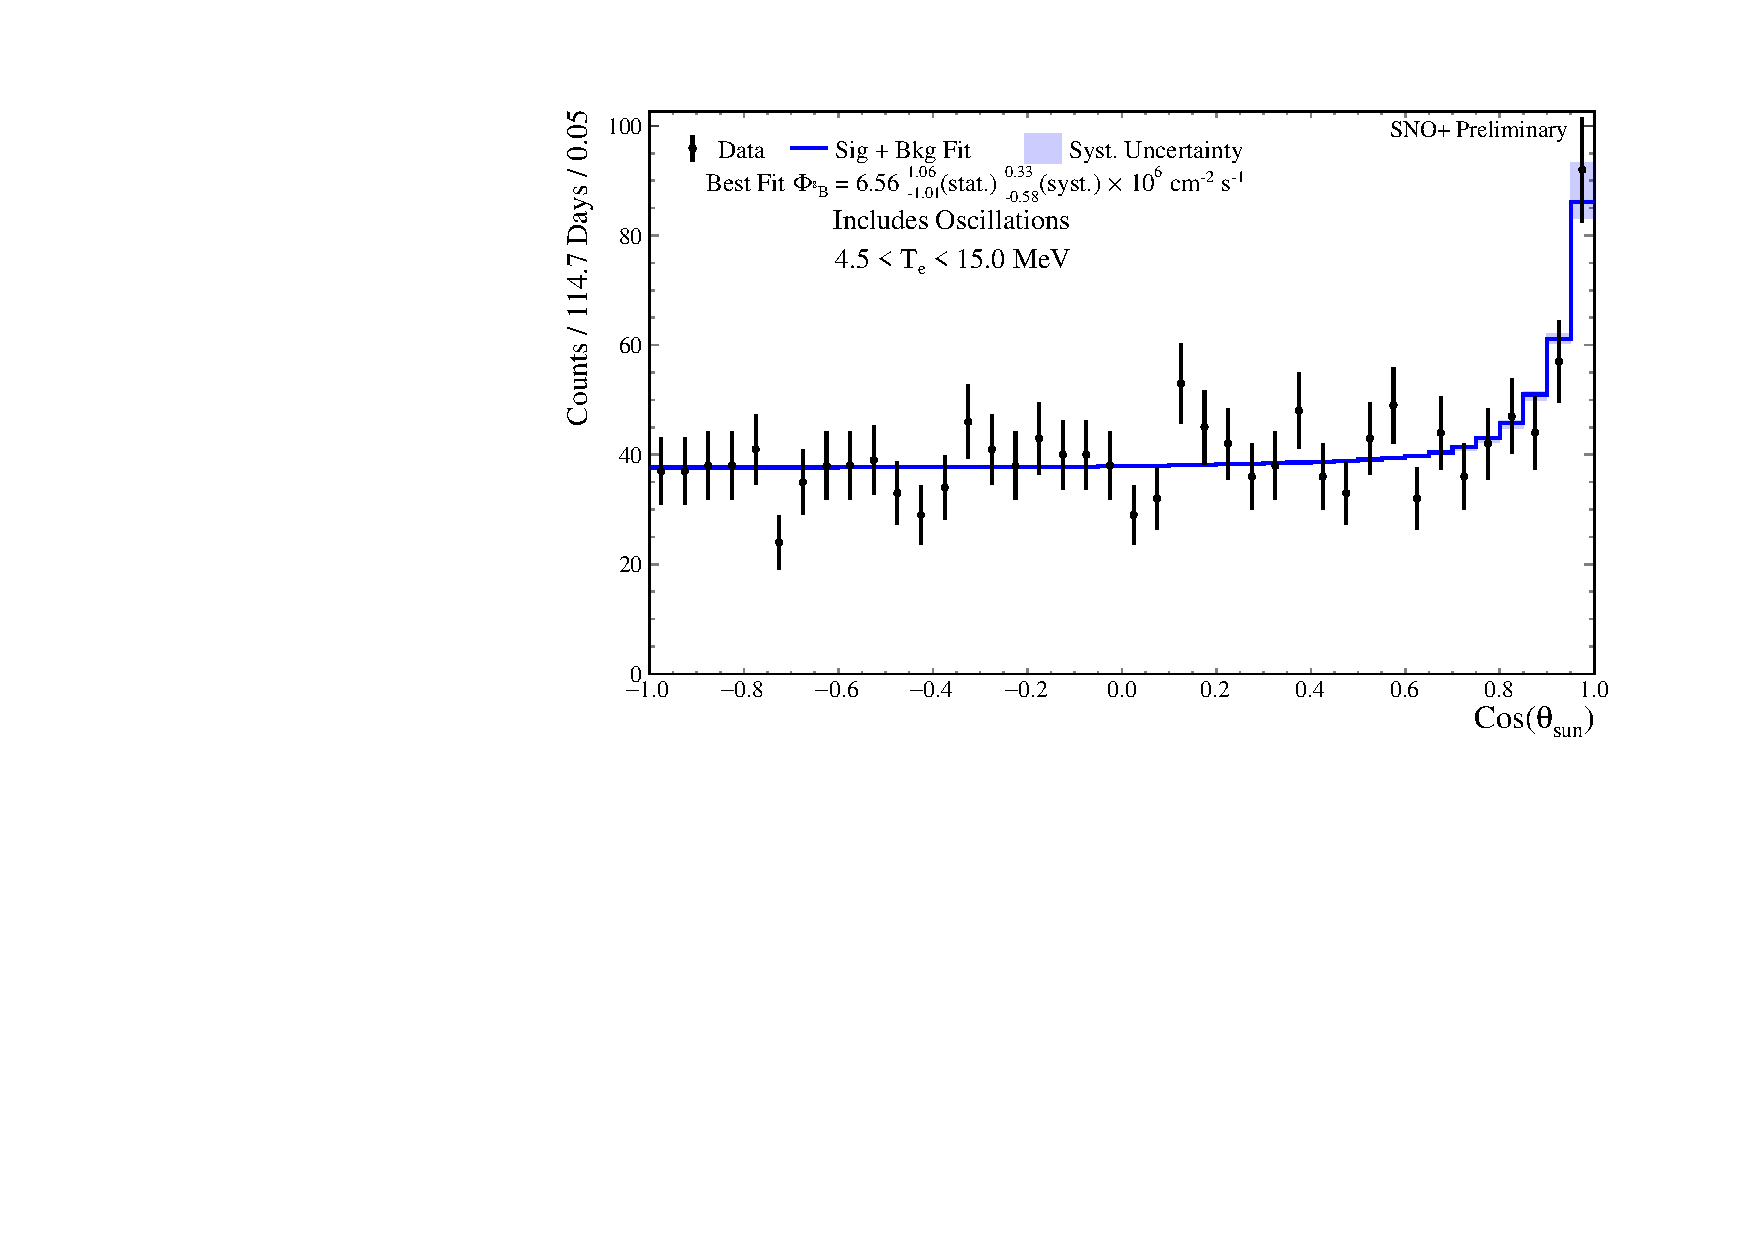
\includegraphics[width=\textwidth]{b8_es_fit_final}
\caption{Summary plot of the $^8B$ ES fit on the unblinded dataset.}
\label{fig:solar:unblind_fit}
\end{figure}


\subsection{Systematic Effects}

Systematics on energy, position, and angular resolution are considered in this 
analysis. 
The energy and position systematics have a negligible effect on the shape of 
the ES PDF, so these systematics are propagated through the expected number of 
ES events. 
The angular resolution systematic has a negligible effect on the effected 
number of events, so it is propagated by distorting the ES PDF in the 
fit yielding a systematic on the fitted number of ES events.
This is described in detail in the following sections with the uncertainties 
and  impact values summarized in Table \ref{tbl:solar:unblind_syst}

With the systematic effects known for the expected and fitted number of ES
events, this is propagated in the usual way to give a systematic on the 
measured flux $^{+0.23}_{-0.58}$ cm$^{-2}$s$^{-1}$.

\begin{equation}
\Phi_{8B,syst} = \Phi_{8B,MC}\frac{N_{fit}}{N_{expected}} \sqrt{
    \left(\frac{N_{expected,syst}}{N_{expected}}\right)^2 +
    \left(\frac{N_{fit,syst}}{N_{fit}}\right)^2
    }
\end{equation}

\begin{table}[]
\begin{center}
\begin{tabular}{c|c|c|c}
Systematic & Uncertainty & Impact & Origin \\ \hline
$E_{scale}$     & $\pm 2.9\%$ & $^{+3.97}_{-3.80}$ events & Logan L. N16 Internal \rule{0pt}{2.6ex}\rule[-1.2ex]{0pt}{0pt}  \\
$E_{res}$       & $10.2\%$ at 5MeV & $\pm0.27$ events & Logan L. N16 Internal  \rule{0pt}{2.6ex}\rule[-1.2ex]{0pt}{0pt}  \\
${XYZ}_{scale}$ & $(^{+0.03}_{-0.19}\%,^{+0.03}_{-0.38}\%,^{+0.03}_{-0.37}\%)$ & $^{+0.62}_{-0.05}$ events & Ed L. N16 Internal  \rule{0pt}{2.6ex}\rule[-1.2ex]{0pt}{0pt}  \\
Dir$_{res}$     &  $\Delta = ^{+0.08}_{-0.19}$ & $^{+10.38}_{-3.58}$ events & Ed L. N16 Internal \rule{0pt}{2.6ex}\rule[-1.2ex]{0pt}{0pt}  \\
$\beta_{14}$ & $\pm 3.1\%$ & $^{+0.50}_{-0.09}$ events & Ryan B. N16 Internal\\ \hline
\end{tabular}
\caption{Systematic effects considered on the unblind data analysis. Note that
    the direction systematic impacts the fitted number of ES events, while
    all others impact the expected number of events. These values can be roughly
    compared to the expected 95.09 ES events.}
\label{tbl:solar:unblind_syst}
\end{center}
\end{table}

\subsubsection{Expected ES Events (Energy and Position)}

The energy scale and resolution were determined by comparing 
internal N16 data to MC. This yielded a $2.9\%$ uncertainty on the energy
scale, and a nominal $10.2\%$ smearing at $5$MeV to be applied to MC to match
the data.
To find the smearing at other energies $E$ in MeV, the following equation was 
assumed
\begin{equation}
\label{eqn:solar:esmear}
E_{smear} = 0.102\sqrt{5 E}.
\end{equation}
To propagate the energy scale systematic, the MC reconstructed energy was 
smeared up and down by $2.9\%$ and recalculating the expected number of events
resulting in  a systematic effect of $^{+0.938}_{-927}$ events. 
The energy resolution systematic was propagated by smearing the MC according to
\ref{eqn:solar:esmear} and recalculated the expected number of events.
The change in expected number of events is assumed to be two-sided and results
in a systematic effect of $\pm1.596$ events.

As the solar MC is simulated as a uniform distribution inside the AV, and the
position resolution is small, smearing the position by this resolution has a 
negligible effect on the expected number of events.
The important position systematic is the vertex scale as this changes the 
fiducial volume.
The vertex scale systematic is determined for each axis by comparing
internal N16 data to MC and found uncertainties of
$(^{+0.03}_{-0.19}\%,^{+0.03}_{-0.38}\%,^{+0.03}_{-0.37}\%)$.
To propagate these systematics the axes were simultaneously scaled up and down
by these values and the expected number of events recalculated in each case.
The change from nominal yields a systematic effect of $^{+0.62}_{-0.05}$.

The total systematic on the expected number of events is found by adding the
systematic effects above in quadrature: $^{+4.03}_{-3.81}$.

\subsubsection{Fitted ES Events (Angular Resolution)}

The angular resolution was determined by comparing internal N16 
data to MC. As mentioned, this systematic does not affect the expected 
number of events, but does strongly affect the shape of the ES PDF as 
described by Equation \ref{solar:eq:dirres}.
The values for $\Delta$ determined from Ed's analysis were $^{+0.08}_{-0.19}$.
The fit was rerun with ES PDFs distorted by these values and the fitted 
number of ES was compared to the nominal non-distorted case.
This resulted in a systematic on the fitted number of ES events of 
$^{+10.38}_{-3.58}$.

\subsection{Result Summary}

The analysis described above yields Figure \ref{fig:solar:unblind_fit} and a 
$^8B$ flux of
$6.56$ $^{+1.06}_{-1.01}$ (stat.) $^{+0.33}_{-0.58}$ (syst.)$\times$cm$^{-2}$s$^{-1}$.
It's worth noting that the error band reflects the uncertainty on the solar
$\nu$ prediction.
That is, it's simply the quadrature sum of the systematics described above,
scaled up to match the best fit solar flux.
The systematic error bar on the solar flux does not directly match that band,
the error bar comes from doing multiple fits to determine the effect each systematic
has on the resulting solar flux.

Recent global fits to solar neutrino data gives a solar flux $^{8}B$ of
$5.16 \times 10^6$ cm$^{-2}$ s$^{-1}$.
This measurement is 1.20 $\sigma$ from that, giving a P-value of $23.0\%$.


\section{Final Analysis}
\label{sec:solar:updated}
The results of the unblinded analysis described above was show at conferences and so that section remains as-is for historical purposes. 
The solar ES results were later deemed worthy of publication and some additional effort was put into this analysis.
The remaining discussion centers around differences from the previous unblind analysis.

Not discussed in detail is a thorough rewriting of the underlying analysis code to be significantly more efficient, however the statement can be made that the new code was vetted to reproduce the previous results.
In the time since the unblinded analysis, a more detailed calculation of data livetime results in a different lifetime for this fit relative to previous fits.
Other changes relative to the previous unblinded analysis are documented in the following sections.


\subsection{Reconstructed Energy}
Comparison of the N16 calibration data to MC demonstrated that the energy reconstruction algorithm was not performing optimally.
From this calibration data an energy correction lookup table applied to both data and MC was derived.
Further analysis of N16 calibration data demonstrated radius- and z-dependent energy scale bias in the energy reconstruction algorithm that was corrected by applying the following scaling to the reconstructed energy
\begin{equation}
1 + A + ( (1 + B \rho^2)(1 + Cz + D*z^2 + Ez^3) - 1 )
\end{equation}
where $A$, $B$, $C$, $D$, and $E$ were determined separately for data and MC.

\subsection{Angular Systematic}
Previously the uncertainty in angular resolution was accounted for with the functional form  \ref{solar:eq:dirres} applied directly the $\cos \theta_{sun}$ PDF. 
For the solar ES analysis this was probably fine, however it was noted that this results in events being pushed into non-physical values ($\cos \theta_{sun} < -1$) or leaving a void of zero probability near $\cos \theta_{sun} = 1$.
To handle this better, it was proposed to instead adjust the reconstructed direction of each MC event to be further or nearer the MC truth direction (as determined by  \ref{solar:eq:dirres}) and finally recomputing the $\cos \theta_{sun}$ PDF using these new directions.
This method was adopted in this analysis.

Additionally, as the angular systematic was the dominate systematic and the solar data well constrains the angular resolution, this analysis opted to float this uncertainty using the shift-and-refit one-$\sigma$ uncertainty as a constraint.
This requires re-smearing each event's direction and rebuilding the angular PDF at each step of the fit which is computationally challenging but tractable for this analysis with so few floated variables.

\subsection{Systematic Propagation}
Previously systematic uncertainties were propagated via their impact on either the expected (most systematic uncertainties) or fitted number of events (only angular systematic). 
This method failed to properly take into account correlated effects from a single systematic uncertainty to the expected and fitted number of events.
These correlated effects are small for the reasons highlighted in the unblinded analysis above, but not negligible.
This analysis improves on the previous by recomputing the solar PDF for each systematic to recalculate the expected number of events and refitting the data with the new PDF to recalculate the fitted number of events.
The fitted solar flux scale - the ratio between fitted and expected events - then contains the impact due to the systematic on both effects.

\subsection{Updated Systematic Uncertainties}
Since the previous analysis the uncertainties on most systematic parameters have been revised. 
Due to low impact the $\beta_{14}$ systematic was dropped.
Both a position resolution and position shift systematic were added, however neither has significant impact.
See Table \ref{tbl:solar:updated_syst} for the values used here.

\begin{table}[]
\begin{center}
\begin{tabular}{c|c|c|c}
Systematic & Uncertainty & Application & Origin \\ \hline
$E_{scale}$     & $\pm 2.0\%$ & shift-refit $^{+0.0217}_{-0.0204}$ & N16 Internal \rule{0pt}{2.6ex}\rule[-1.2ex]{0pt}{0pt}  \\
$E_{res}$       & $\sqrt{(1+0.0018)^2-1.0}\sqrt{E}$ & shift-refit $\pm 0.0005$ & N16 Internal  \rule{0pt}{2.6ex}\rule[-1.2ex]{0pt}{0pt}  \\
${XYZ}_{scale}$ & $(^{+0.91}_{-1.01},^{+0.92}_{-1.02},^{+0.91}_{-0.99}) \%$ & shift-refit $^{+0.0261}_{-0.0284}$ & N16 Internal  \rule{0pt}{2.6ex}\rule[-1.2ex]{0pt}{0pt}  \\
${XYZ}_{shift}$ & $(^{+16.4}_{-18.2},^{+22.3}_{-19.2},^{+38.4]}_{-16.7})$ mm & shift-refit $^{+0.0002}_{-0.0001}$ & N16 Internal  \rule{0pt}{2.6ex}\rule[-1.2ex]{0pt}{0pt}  \\
${XYZ}_{res}$ & $(104.0,98.2,106.2)$ mm & shift-refit $\pm 0.0002$ & N16 Internal  \rule{0pt}{2.6ex}\rule[-1.2ex]{0pt}{0pt}  \\
Dir$_{res}$     &  $\Delta = ^{+0.08}_{-0.13}$ & floated (best fit $\Delta = -0.02^{+0.09}_{-0.13}$) & N16 Internal \rule{0pt}{2.6ex}\rule[-1.2ex]{0pt}{0pt}  \\ \hline
\end{tabular}
\caption{ Systematic uncertainties considered on the updated solar ES analysis are shown here. 
The impact shown for shift-and-refit parameters is a fractional change of the $^8$B flux from the central value of the fit for the energy range $4.5-15.0$ MeV.
For the livetime considered in this analysis approximately 100 solar ES events are expected.}
\label{tbl:solar:updated_syst}
\end{center}
\end{table}


\subsection{Result Summary}

\begin{figure}
\centering
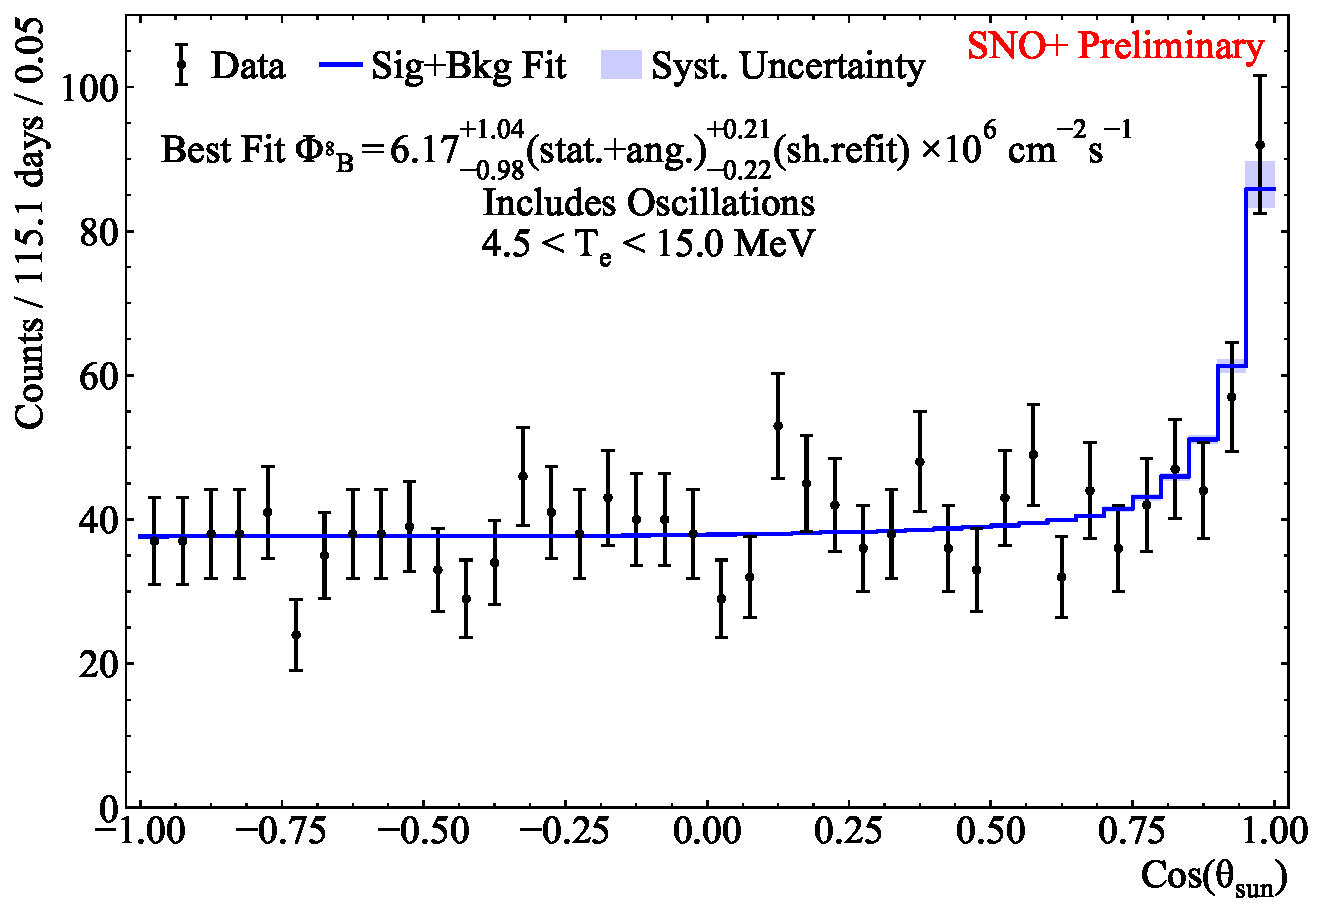
\includegraphics[width=\textwidth]{8b_es_4_5_15_0_fit_float_ang_res}
\caption{Summary plot of the updated $^8B$ ES analysis on the unblinded dataset using the energy range $4.5-15.0$ MeV.}
\label{fig:solar:unpdated_fit_4.5}
\end{figure}

Using the previously unblinded solar data, the full energy range $4.5-15.0$ MeV can be fit. 
The results of this fit is shown in Figure \ref{fig:solar:unpdated_fit_4.5} and can be found in \cite{snoplus_solar}.
Notably this fit is consistent with the current global best fit for the $^8$B neutrino flux, and demonstrates that SNO+ has achieved very low backgrounds as evidenced by the clear ES peak in the solar direction.
